\documentclass[12pt]{article}

% If you're new to LaTeX, here's some short tutorials:
% https://www.overleaf.com/learn/latex/Learn_LaTeX_in_30_minutes
% https://en.wikibooks.org/wiki/LaTeX/Basics

% Formatting
\usepackage[utf8]{inputenc}
\usepackage[a4paper,width=150mm,top=25mm,bottom=25mm]{geometry}
\usepackage{titlesec}
\usepackage{enumitem}
\usepackage[english]{babel}
\usepackage{fancyhdr}
\usepackage{hyperref}

% \geometry{
%     a4paper,
%     total={170mm,257mm},
%     left=20mm,
%     right=20mm,
%     top=0mm,
% }

% Math
% https://www.overleaf.com/learn/latex/Mathematical_expressions
% https://en.wikibooks.org/wiki/LaTeX/Mathematics
\usepackage{amsmath,amsfonts,amssymb,mathtools}

% Images
% https://www.overleaf.com/learn/latex/Inserting_Images
% https://en.wikibooks.org/wiki/LaTeX/Floats,_Figures_and_Captions
\usepackage{graphicx,float}
\usepackage{caption}
\usepackage{subcaption}

% Tables
% https://www.overleaf.com/learn/latex/Tables
% https://en.wikibooks.org/wiki/LaTeX/Tables

% Algorithms
% https://www.overleaf.com/learn/latex/algorithms
% https://en.wikibooks.org/wiki/LaTeX/Algorithms
\usepackage{algorithmic}

% Tikz for drawing graphs and diagrams, although using other tools and 
% importing images might be easier
% This gives a pretty good tutorial: 
% http://www.tcs.uni-luebeck.de/downloads/mitarbeiter/tantau/2012-gd-presentation.pdf
\usepackage{tikz}


% Title content
\title{\textbf{Heart Problem Predictor}}
%\author{\small Arielle Soomi Yoo, Samuel Robert Perelgut, Catherina Castillo, Mia Ma, William T Wu, Aashir Shukla, Derek Li}
\author{}
\date{}
\pagestyle{fancy}
\fancyhf{}
\rhead{ECS 171 SQ 2021}
\lhead{Group 13 Final Report}
\rfoot{\thepage}

\begin{document}
\titlespacing*{\section}{0pt}{0.25cm}{0.25cm}
\titlespacing*{\subsection}{0pt}{0.5cm}{0.5cm}
\maketitle

\section*{Introduction}

\subsection*{}
In the age of machine learning and big data, we have many tools at our 
disposal for prediction, especially in health. From predicting the 
likelihood of getting a disease to classifying what kind of disease a 
person has, machine learning can help doctors and researchers better 
diagnose and make decisions on how to treat their patients. Further, a few 
past studies on the matter have shown that in some cases artificial 
intelligence programs have superior judgement when making these decisions 
then medical professionals do [1]. Also, artificial intelligence in 
healthcare can have important applications in healthcare because of 
its ability to use very complex data, learn from it, find the most 
important features of the data, and deliver recommendations [5]. 
That is not to say that machine learning algorithms are superior to or a 
replacement for a doctor, but rather it is a reliable extra tool available 
to them that will help them ensure the best outcome for their patients 
with less subjective bias. While we are only focusing on heart disease 
for our project, our general topic covers the important intersection 
between human health and machine learning.
The overall purpose of this project is to create a website that can assist 
medical professionals in diagnosing whether a patient is at risk for heart 
disease with a machine learning backend. The main machine learning 
algorithms we considered for this project were logistic regression 
and random forest, since these are both popular algorithms to perform 
classification. In general, as a team we had two subteams, one working on 
backend and another working on frontend, to help finish this project 
together. We were able to try both logistic regression and random forest, 
compare the results, and finalize our web application to launch our chosen 
machine learning algorithm such that the user can input their data to get 
a prediction for health disease risk using UCI data [2, 3].
In this report, we have performed a literature review describing both 
logistic regression and random forest, a dataset description, our 
proposed solution and experimental results. For the literature review, 
we explain the equations involved in logistic regression and random forest,
the equations involved, and how it has been used in the past on health 
data. For the dataset description, we detail how the data was collected 
for each of the features [2, 3]. In our proposed solution and experimental 
results, we explained how we chose to evaluate our models, showed our 
results from model evaluation, and explained the creation of the user 
interface of our web application including how it is organized in a 
model-view-controller software design pattern [4].

\newpage
\section*{Literature Review}

\subsection*{}
When considering different machine learning algorithms for classification of the patient data into either having heart disease risk or not, we thought of using logistic regression because we already had some experience from class and it seemed like a very good simple model to start with. In general, logistic regression works by forming a weighted sum of the input data and using an activation function, such as the sigmoid function, to make a prediction. Weights are found by formulating the logistic regression as a maximum likelihood estimation and then using gradient descent. The original dataset has 3 papers related to it published around 1989 [listed in 6], and of the two we could access, one used logistic regression for predicting heart disease [3] while the other focused on top-down hierarchical clustering to find clustering rules [7]. Since we are primarily interested in performing prediction and the original paper for prediction focuses on logistic regression, this confirmed our belief that logistic regression could be a good tool to use on this dataset. Also, we learned from class that logistic regression is less sensitive to outliers and less sensitive to the selected threshold value for classification than linear regression. Thus, we hope that logistic regression will work well on our data. 
	The other machine learning algorithm we considered was random forest. Random Forest is a machine learning algorithm that uses a combination of many tree classifiers where each tree is formed by randomly partitioning the data and each tree votes on what the correct prediction for the data should be [8]. In general, we were interested in using random forest classifiers because it seems like random ensemble classifiers are generally more accurate than individual classifiers that can make up an ensemble classifier [8]. Also, in a paper comparing logistic regression with classification and regression tree (CART) for predicting heart disease, which is similar to random forest except this classifier partitions based on purity score instead of partitioning many times randomly [10, 11], CART and logistic regression both perform well [9]. However, logistic regression assumes that dependent variables are independently and randomly sampled [9], while generally random forest and CART do not make any assumptions about the underlying distribution of the data [9, 11]. Additionally, random forest works well on imbalanced data and can help estimate the importance of variables used in classification [11]. Because of this information, we hoped that our random forest classifier would have better accuracy than the logistic regression classifier. While we have not directly discussed random forest in class, we have used isolation forest for outlier detection and have discussed decision trees as of week 7. This required a bit of outside learning on our part, but we thought the potential increase in accuracy in using random forest was important enough to investigate.

\section*{Dataset Description}
\subsection*{}
The data for this project originally comes from The UCI Machine Learning Repository and contains data with 76 attributes donated from four different medical sources [2, 3].  We downloaded the 14 variable subset directly from the kaggle website, which has some more information on this UCI dataset [2, 3]. In general, the 14 variables we focused on include general background information on the 303 patients, various cardiac health measurements taken from the patients, and the presence or absence of heart disease [2, 3]. 
Our 13 independent variables include sex, chest paint type, fasting blood sugar, resting electrocardiographic results, exercise induced angina, the slope of the peak exercise ST segment, number of major vessels colored by flourosopy, thalassemia, age in years, resting blood pressure, serum cholestoral, maximum heart rate achieved, and ST depression induced by exercise relative to rest. 8 of these 13 independent variables are categorical variables that are already encoded and 5 are numerical variables. Our dependent variable is a binary categorical variable of angiographic disease status, 1 is for higher than 50\% diameter narrowing and 0 is for less than 50\% diameter narrowing. From this data, we should be able to predict whether a patient is at risk of heart disease or not. 
In the data cleaning process, we found and removed 7 invalid data, which is about 2\% of the original dataset. By invalid, it means they have entries that are out of range. For instance, “thal” is a categorical variable that ranges from 1 to 3 , but the 48th row has 0 for “thal”, which cannot be correctly interpreted and from what we can tell represents missing data. Therefore, removed. We have also removed 9 outliers, which is about 3\% of the original dataset, according to the intersection of Isolation Forest and Local Outlier Factor methods. We have removed 16 rows of data totally, which is about 5\% of the original dataset, and we are left with 287 clean data to analyze. 
We splitted the dataset into 3:7 testing dataset and training dataset for further classification algorithms.
\begin{center}
    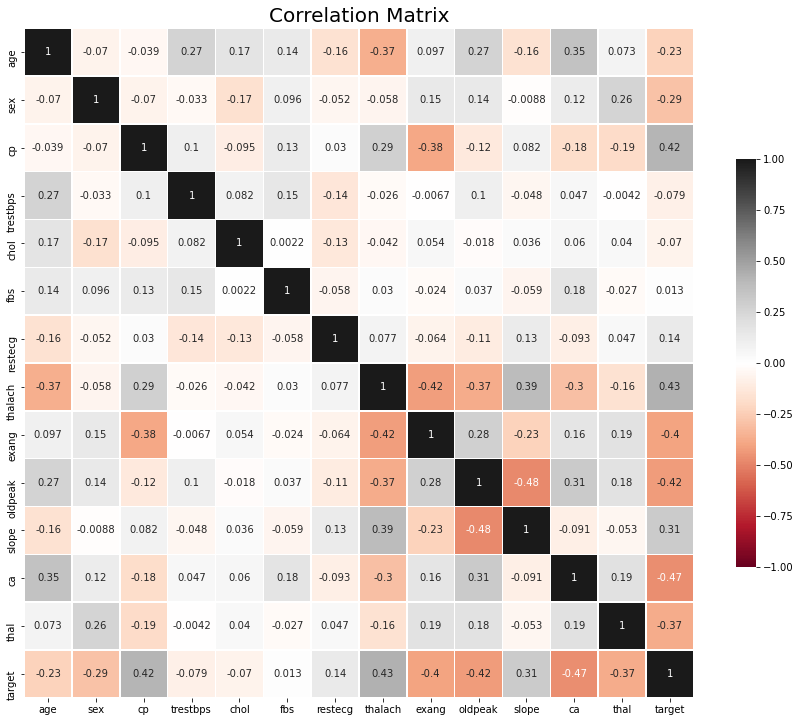
\includegraphics[width=\textwidth, height=12cm, keepaspectratio]{images/image5.png}
\end{center}


According to the correlation matrix, there is no significant correlation between independent variables.
We  also found some interesting relationships between age, sex and risk of heart diease in the explortory data analysis.
\begin{center}
    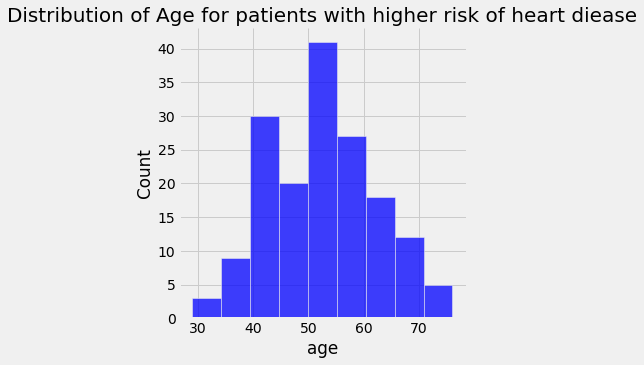
\includegraphics[width=\textwidth, height=10cm, keepaspectratio]{images/image2.png}
\end{center}

People ages from 50 to 55 have the highest proportion in this higher risk sample population, which means a person is most likely to have heart disease in their 50s. People in their 30s and 70s both have the lowest proportion in this sample population, but probably for different reasons: 30-ish people are generally healthier, but not everyone can make it to their 70s, so 70s is an overall smaller population 
\begin{center}
    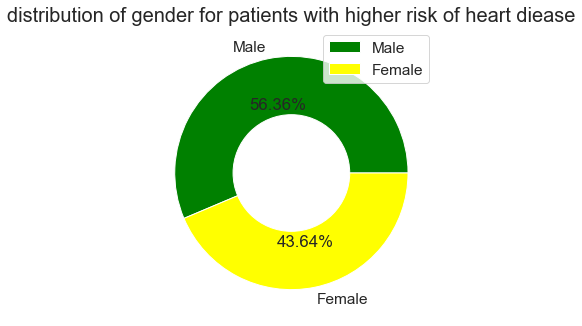
\includegraphics[width=\textwidth, height=10cm, keepaspectratio]{images/image1.png}    
\end{center}
In the higher risk population , 56.36\%  are male patients and  43.64\% are female patients. Males patients are 12.72\% more than female patients. 

\section*{Proposed Solution and Experimental Results}
\subsection*{Solution Overview:}
We are interested in producing a web application that can accurately produce a prediction for heart disease from user input using a machine learning model. The overall process we implemented was first processing our dataset by removing outliers, splitting it, and normalizing the values. Next we trained the model on the dataset and ported it over to a simple file that can be used at runtime for when the user enters their input. Lastly we take the user input and use the model to predict whether they are at risk for heart disease. Obvious obstacles we had to overcome were creating the model as well as an interface for it, displaying the users results, and picking the best algorithm. 

A Logistic Regression model determines categorical dependent variables on the basis of independent variables. It is similar to Linear Regression, with the addition of the Sigmoid Activation Function, which contains values between 0 and 1: 
$$S(x) = \frac{1}{1+e^x}$$
This is suitable for our problem as we would like to predict heart disease, which is either 0 (which implies no heart disease) or 1 (there is a heart disease). It also has a different cost function from linear regression. Gradient Descent was run to minimize this cost function. Finally, values can be predicted using this model by using the following formula:
$$log(\frac{p}{1-p}) = \beta_0 + \beta_1x_1 + \beta_2x_2 + \beta_3x_3 + \dots$$
Where P is the probability of heart disease, represents the model coefficients, and xrepresents the features.

We decided to test the dataset using a model trained on Logistic Regression as well as Random Forest. Although the Logistic Regression model has a higher mse compared to the Random Forest model, we stuck to Logistic Regression. We decided to stick to Logistic Regression based on the fact that the Random Forest model would have a much lower accuracy on the test data.


\subsection*{Model Evaluation}
Since the final model is solely used for classification, evaluating the accuracy of the model is extremely important. Further specifying with the precision and recall scores will more accurately portray the performance of the model. As such, it follows that the comparison of the two algorithms we decided to implement, logistic regression and random forest, required the best scores in precision and recall within reasonable bounds. The mean squared error of the two models was also calculated as a general indication of performance and evaluation of the model resulted in the following metrics:

% precision/recall scores of logistic and forest
\begin{center}
        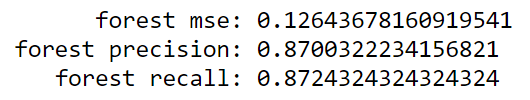
\includegraphics[width=\textwidth, height=\textheight, keepaspectratio]{images/image3.png}
        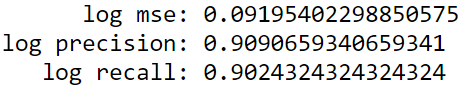
\includegraphics[width=\textwidth, height=\textheight, keepaspectratio]{images/image4.png}
\end{center}

The logistic regression model consistently outperformed the random forest model across many variations of the training and testing sets. This trend was consistent with ROC curves created with the models with the curve created by the logistic regression model slightly outperforming the random forest model with an AUC of 0.9 compared to 0.87 respectively. The confusion matrices quantify the specific performance statistics by the true and false positive/negative results and solidify the decision to proceed with the logistic regression model.

% confusion matrices
\begin{center}
    \begin{figure*}
        \begin{subfigure}{.8\textwidth}
            \centering
            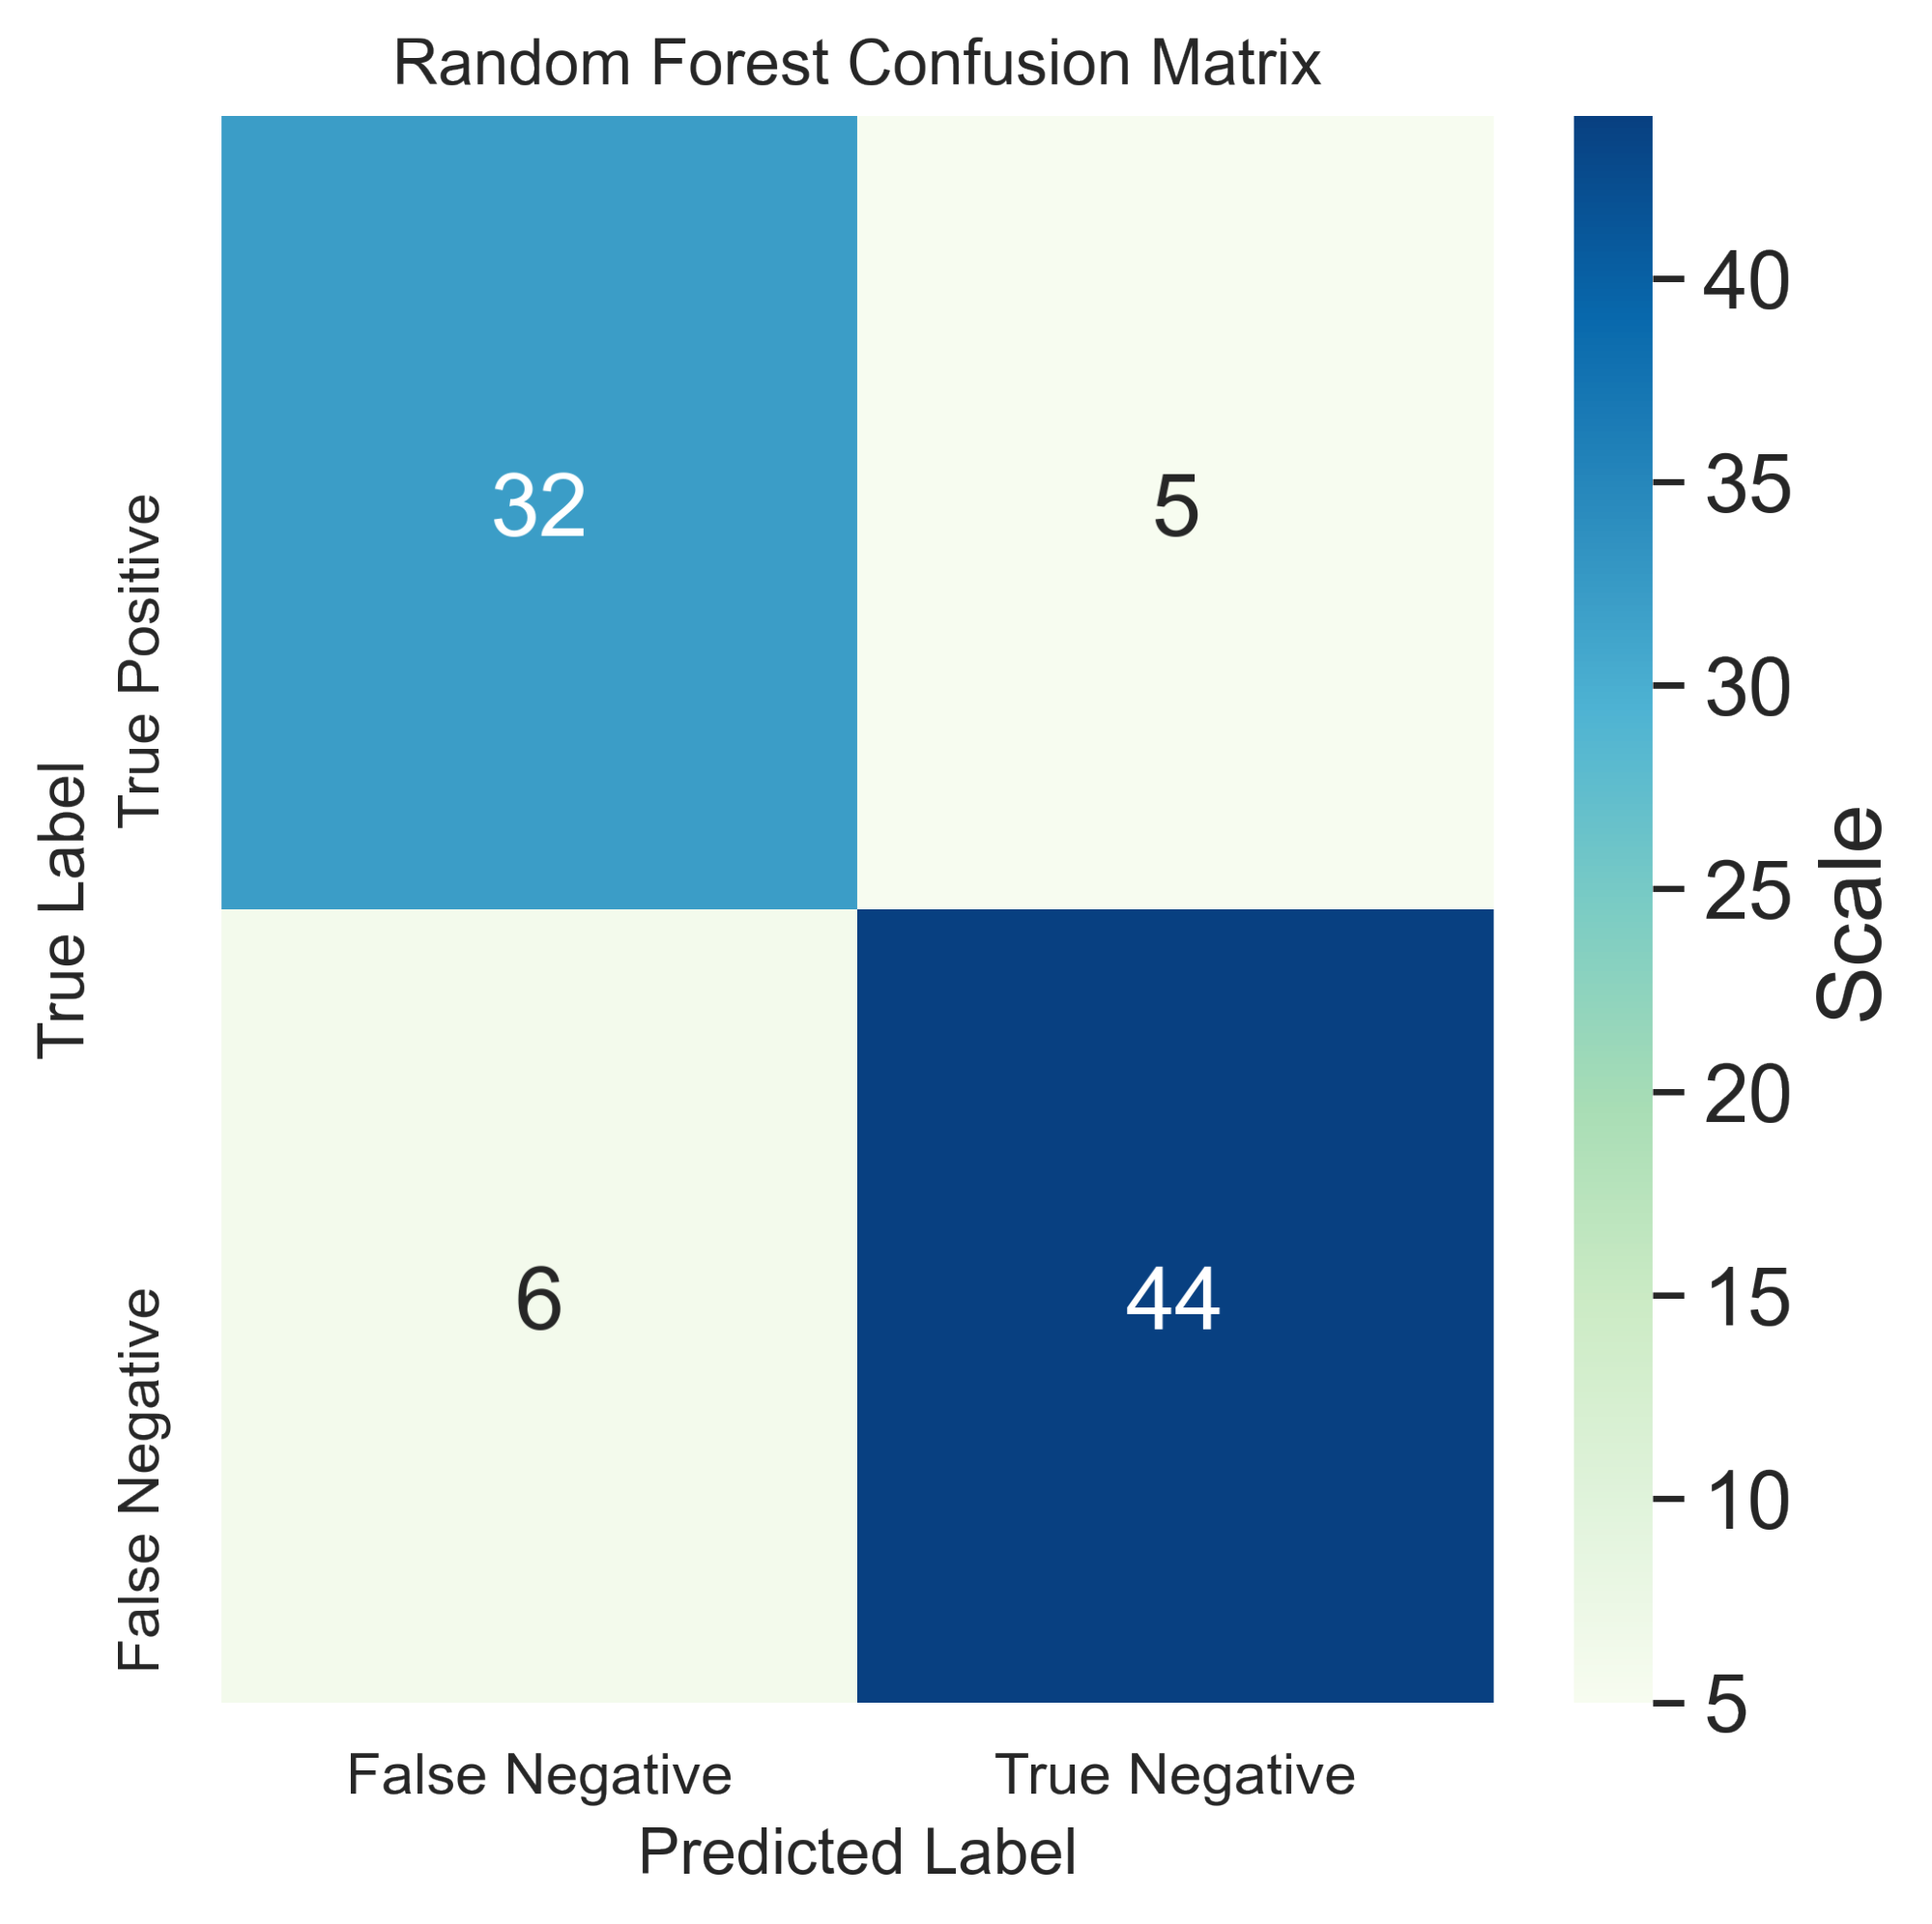
\includegraphics[width=0.5\textwidth, height=0.6\textheight, keepaspectratio]{images/image6.png}
        \end{subfigure}
        \begin{subfigure}{.8\textwidth}
            \centering
            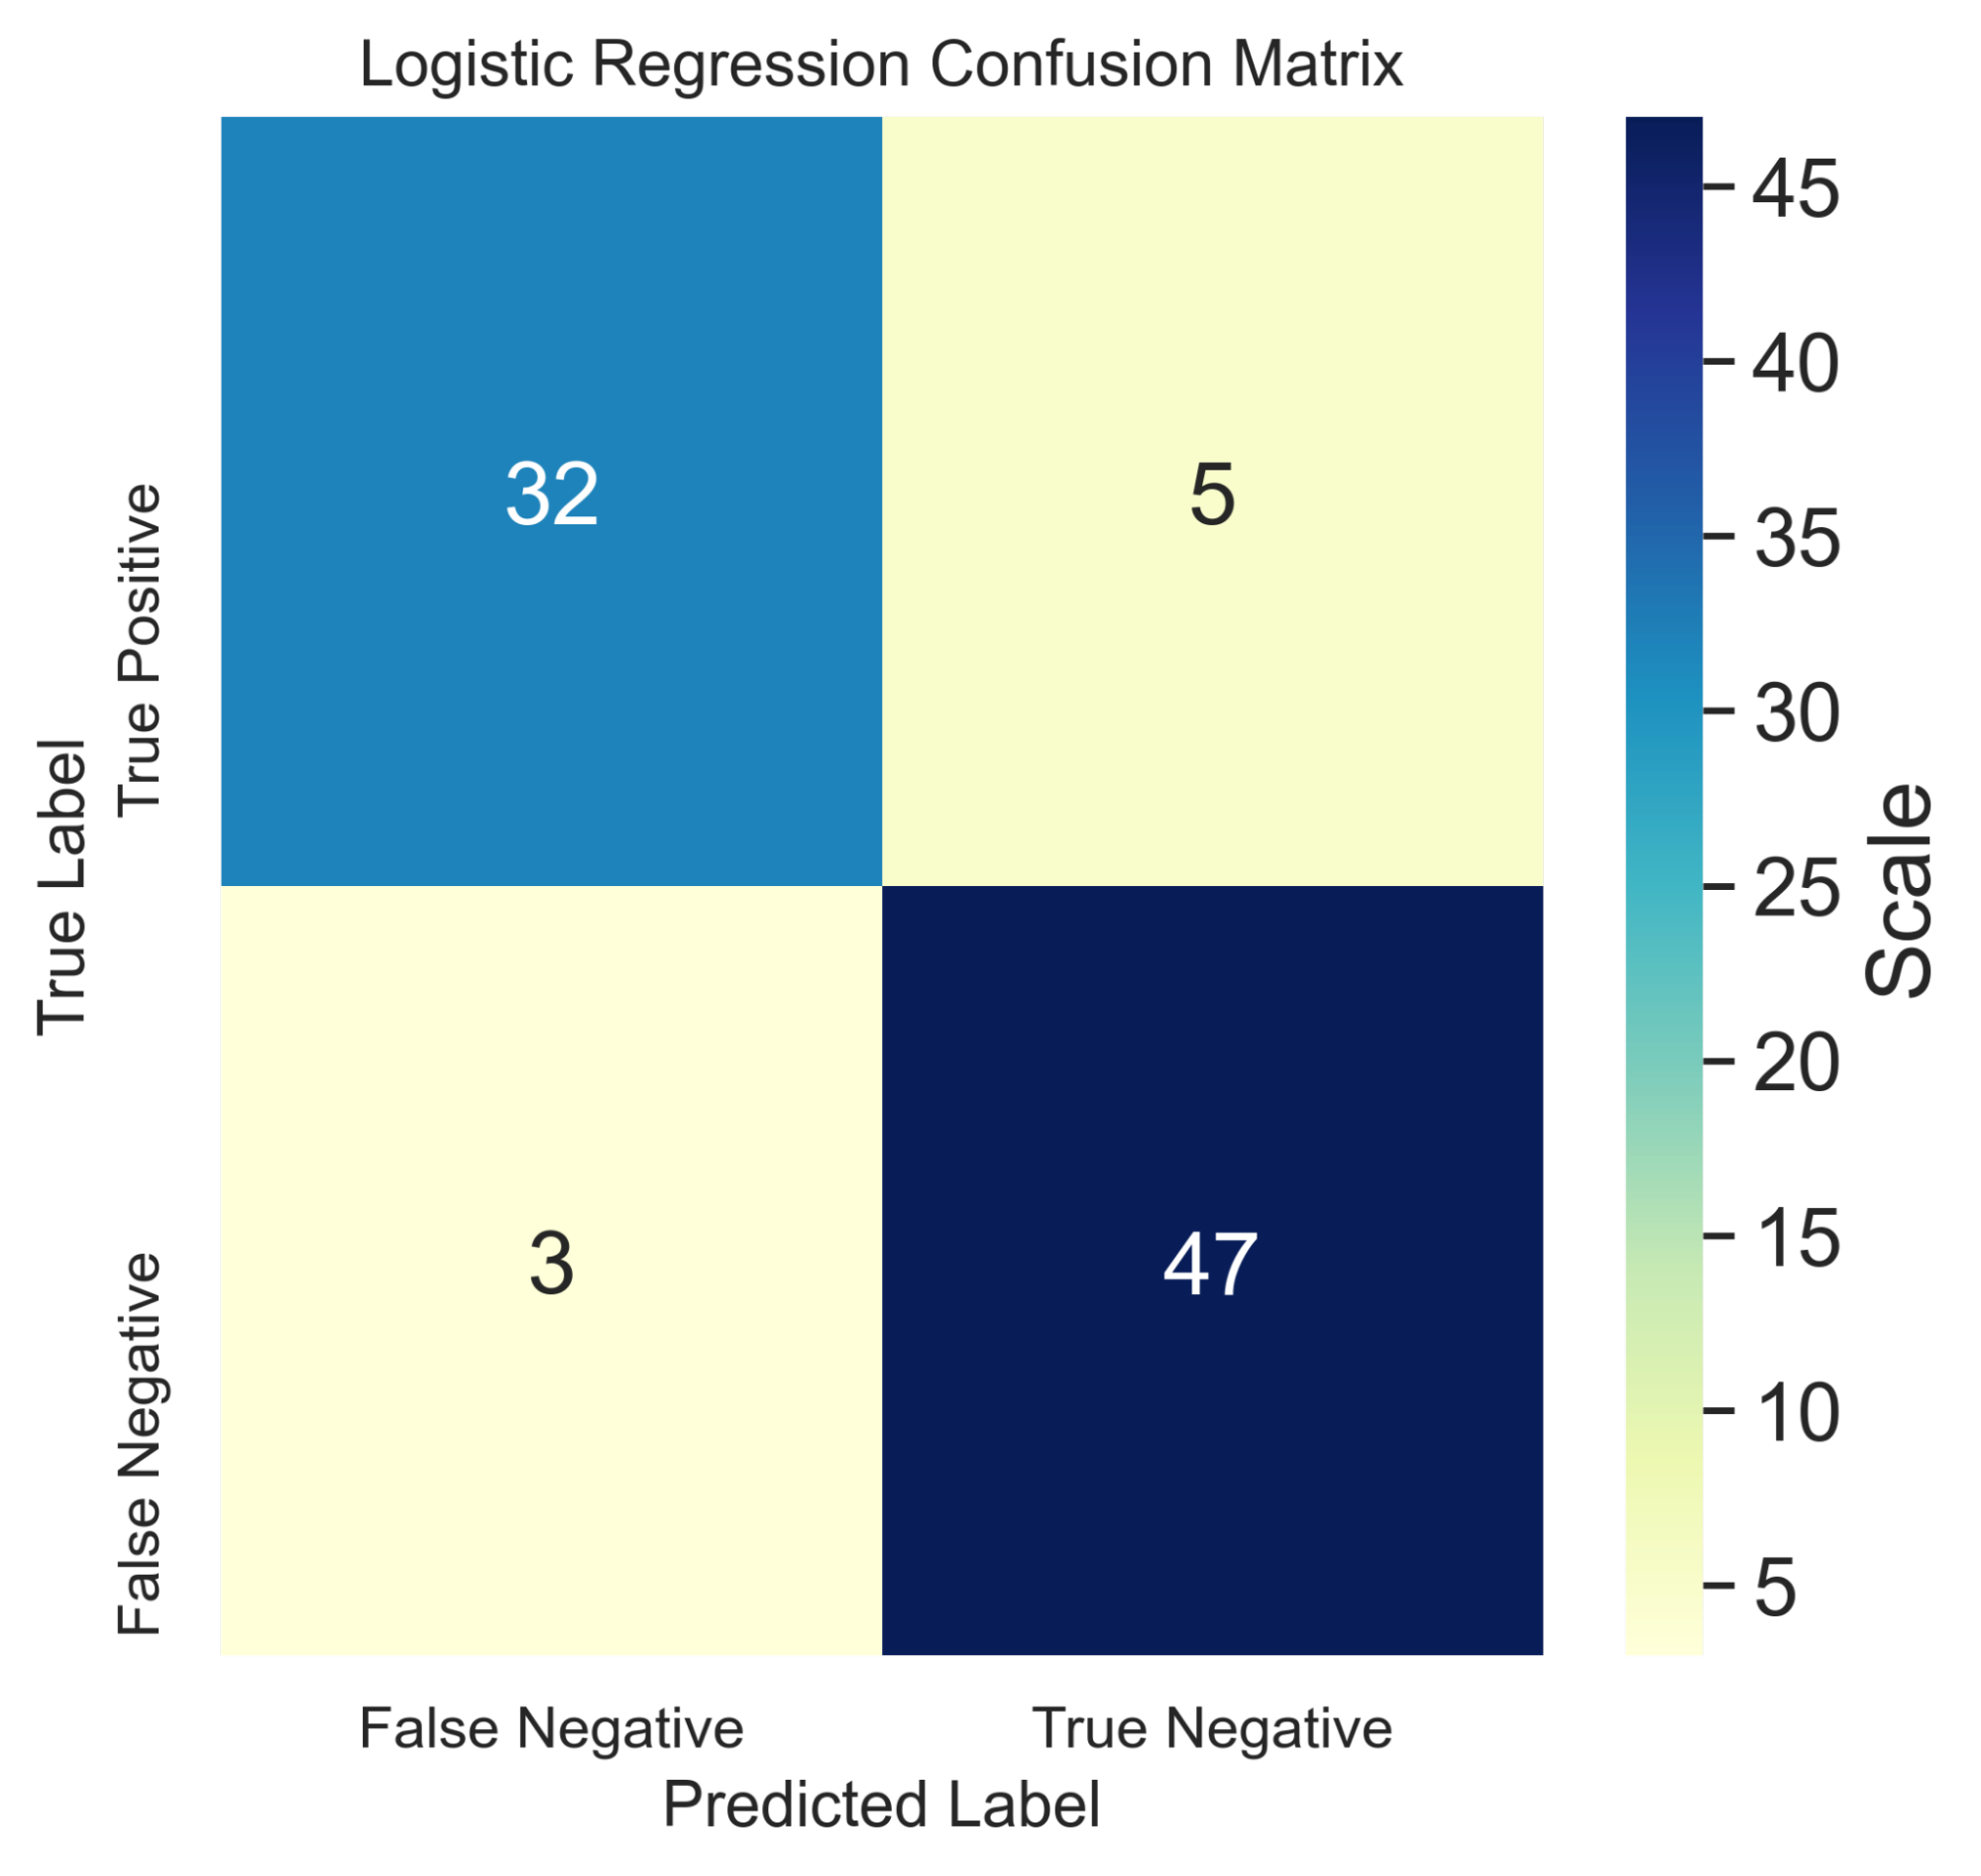
\includegraphics[width=0.5\textwidth, height=0.6\textheight, keepaspectratio]{images/image7.png}
        \end{subfigure}
    \end{figure*}
\end{center}

\section*{User Interface}
\subsection*{}
For the framework of our website, we opted to use HTML, CSS and Jquery for the client-side pages. For our server or controller file, we felt Flask was the optimal choice. We had explored a few options, namely NodeJs, Django, and Flask, but ultimately chose Flask as it was the most similar to Python and had more flexibility with what type of data it can receive and send to other scripts. This second trait was especially important, as we had not decided how our web app would interact and communicate with the machine learning model at the time we were choosing a framework. In conclusion, Flask was chosen because it seemed to be the most versatile, had better guarantees of compatibility with any model the Machine Learning team developed, and allowed the frontend members, who are mostly familiar with HTML, to easily develop a website, without needing to learn a new language or python-based framework. 
	Upon examining the features of the dataset, we felt that it would be best to develop our website from the perspective that our client was a medical professional entering in data about a patient. When loading up the site, the user is presented with several input boxes that correspond to the independent variables our model uses to determine the target variable, the presence of heart disease. When the user is done entering the relevant information, they press the submit button. This causes a jQuery script to take the information from the input boxes, create a JSON from the information, and use an Ajax POST request to send it to our server file, which is again written using Flask. In the server file, we want to take the JSON retrieved from the Ajax request, modify it by putting it into a dictionary, and input it into our model to get the predicted value of the target variable. The backend/machine learning side will have run their model on our dataset and saved the resulting weights to a new file. Our server file will load these weights into a new model, and then use our model to evaluate the user input. When we have our result, the server will package that in a JSON and send it back to the client-side, where it will be displayed below the submission form.
	We implemented some other information-- namely visualization of the target variable distribution and the user's place in those distributions. These graphs were also created by the backend and sent to the frontend by our server.

\section*{Conclusion and Future Direction}
\subsection*{}
Some challenges specifically for the frontend was learning about web development. Most of the members of our team had little experience in Flask, HTML, CSS, and JQuery, which involved specific coding languages or functions that we had never seen before. Catharina Castillo and William Wu both had experience with HTML and CSS, but Flask and JQuery were new for everyone. This resulted in a bit of a learning curve for everyone, especially with regards to learning how to use Flask to both integrate with HTML, CSS, and JQuery as well as with Python, despite it being a Python-based framework.. In general, we had to lean on Catharina on our team because she had the most experience with web development. We are very grateful that we had someone familiar with these kinds of frameworks, but it made trying to split up work evenly difficult as she had to do the bulk of the set up. Fortunately, Arielle Yoo and William Wu were able to catch on well enough to handle a lot of the post-setup coding, for example, expanding inputs to represent the dataset properly, as well as web-styling.
	On the backend side of things, the programming process proceeded without much issue, however, this changed when it came time to integrate the backend code with the front end. Specifically , one of the major obstacles was providing the front end with a fitted model and processed dataset without having to calculate these values each time the website is used. In order to solve this problem we used a library called pickle which writes models to a file so that we could fit the model statically and then pass read it in at run time. On the dataset side of things the problem was not as easy to solve. This is because we needed both the processed and unprocessed data at run time. We use the processed data to create graphs with the user input dynamically, while we use the raw data to normalize the users input so that it is compatible with the fitted model. The solution we went with was to pass in a partially processed dataset and then finish the processing dynamically. This allowed us to both normalize the user input and use the data for graphing while only using a single dataset.  
While our project already provides a useful service that medical professionals could use to help save human lives, there are still many more useful and interesting innovations that us or an entirely different group could add to it in the future. Firstly even though we only considered logistic regression and random forest for our algorithm this is by no means the only option. For example, a neural network with the right parameters may yield even better results than our model did. On the front end side of things, the website itself is not all that complex and there are plenty of ways we could improve the design to improve its aesthetic. The website only consisted of a few text boxes and some graphs, however, it could also provide additional information related to heart problems. Such as how to prevent and deal with them. On a much grander scale, this website could be integrated with others like it to create a program that ensures overall patient healthiness by giving them a diagnosis on a wide array of health issues.
Our project page can be found at \url{https://github.com/cat-castle-99/ECS171Proj}

\newpage
\begin{center}
    \textbf{Works Cited}
\end{center}

\begin{enumerate}
    \item Lysaght, T., Lim, H.Y., Xafis, V. et al. AI-Assisted Decision-making in Healthcare. ABR 11, 299–314 (2019). \url{https://doi.org/10.1007/s41649-019-00096-0}
    \item Ronit. “Heart Disease UCI.” Kaggle, 25 June 2018, \\ \url{www.kaggle.com/ronitf/heart-disease-uci}.
    \item Detrano, R., Janosi, A., Steinbrunn, W., Pfisterer, M., 
    Schmid, J., Sandhu, S., Guppy, K., Lee, S., \& Froelicher, V. 
    (1989). International application of a new probability algorithm 
    for the diagnosis of coronary artery disease. American Journal of 
    Cardiology, 64,304--310. \\ \url{https://www.sciencedirect.com/science/article/pii/0002914989905249?via%3Dihub}
    \item Pop, Dragos-Paul, and Adam Altar. “Designing an MVC Model for Rapid Web Application Development.” Procedia Engineering, Elsevier, 25 Mar. 2014, \\ \url{www.sciencedirect.com/science/article/pii/S187770581400352X}.
    \item Bini, Stefano A. “Artificial Intelligence, Machine Learning, Deep Learning, and Cognitive Computing: What Do These Terms Mean and How Will They Impact Health Care?” The Journal of Arthroplasty, Churchill Livingstone, 27 Feb. 2018, \\ \url{www.sciencedirect.com/science/article/pii/S0883540318302158}
    \item UCI Machine Learning Repository: Heart Disease Data Set, \\ \url{https://archive.ics.uci.edu/ml/datasets/Heart+Disease/}
    \item Gennari, John H., et al. “Models of Incremental Concept Formation.” Artificial Intelligence, Elsevier, Sept. 1989, \\ \url{www.sciencedirect.com/science/article/pii/0004370289900465}.
    \item M. Pal (2005) Random forest classifier for remote sensing classification, International Journal of Remote Sensing, 26:1, 217-222, DOI: 10.1080/01431160412331269698 \\
    \url{https://www.tandfonline.com/doi/full/10.1080/01431160412331269698?casa_token=uzMXfL0QedgAAAAA%3AlPhsBxS-K20fWRnI9BT1DI_PfZe5zXHlFDLrhmlEoER9MG2G3bgdDQ-39KlJqnxvAAi3_Ym7bx0}
    \item Kurt, Imran, et al. “Comparing Performances of Logistic Regression, Classification and Regression Tree, and Neural Networks for Predicting Coronary Artery Disease.” Expert Systems with Applications, Pergamon, 10 Oct. 2006, \\ \url{www.sciencedirect.com/science/article/pii/S0957417406002855?casa_token=zXAY3V78ua8AAAAA%3AYAykd-8uDPDBiAOc1iuk0XaHpyjuQmnazj1E7_Wuk5cbGlxF_9y75W2wXivnxns_eTgPeI9_}
    \item Austin, Peter C., et al. “Using Methods from the Data-Mining and Machine-Learning Literature for Disease Classification and Prediction: a Case Study Examining Classification of Heart Failure Subtypes.” Journal of Clinical Epidemiology, Pergamon, 4 Feb. 2013, \\ \url{www.sciencedirect.com/science/article/pii/S0895435612003551?casa_token=GTuNPBwijyAAAAAA%3AWByDc2H_WHbxrtoKe3n1mxz7oKhiDi9RSFxSPcP0OaLxC9g8tALRz5OhbC-mx6BIYY7YOP1H\#bib15}.
    \item Khalilia, Mohammed, et al. “Predicting Disease Risks from Highly Imbalanced Data Using Random Forest.” BMC Medical Informatics and Decision Making, BioMed Central, 29 July 2011, \url{https://link.springer.com/article/10.1186/1472-6947-11-51}.
\end{enumerate}

\end{document}